\begin{figure*}[t!]
 \begin{center}
  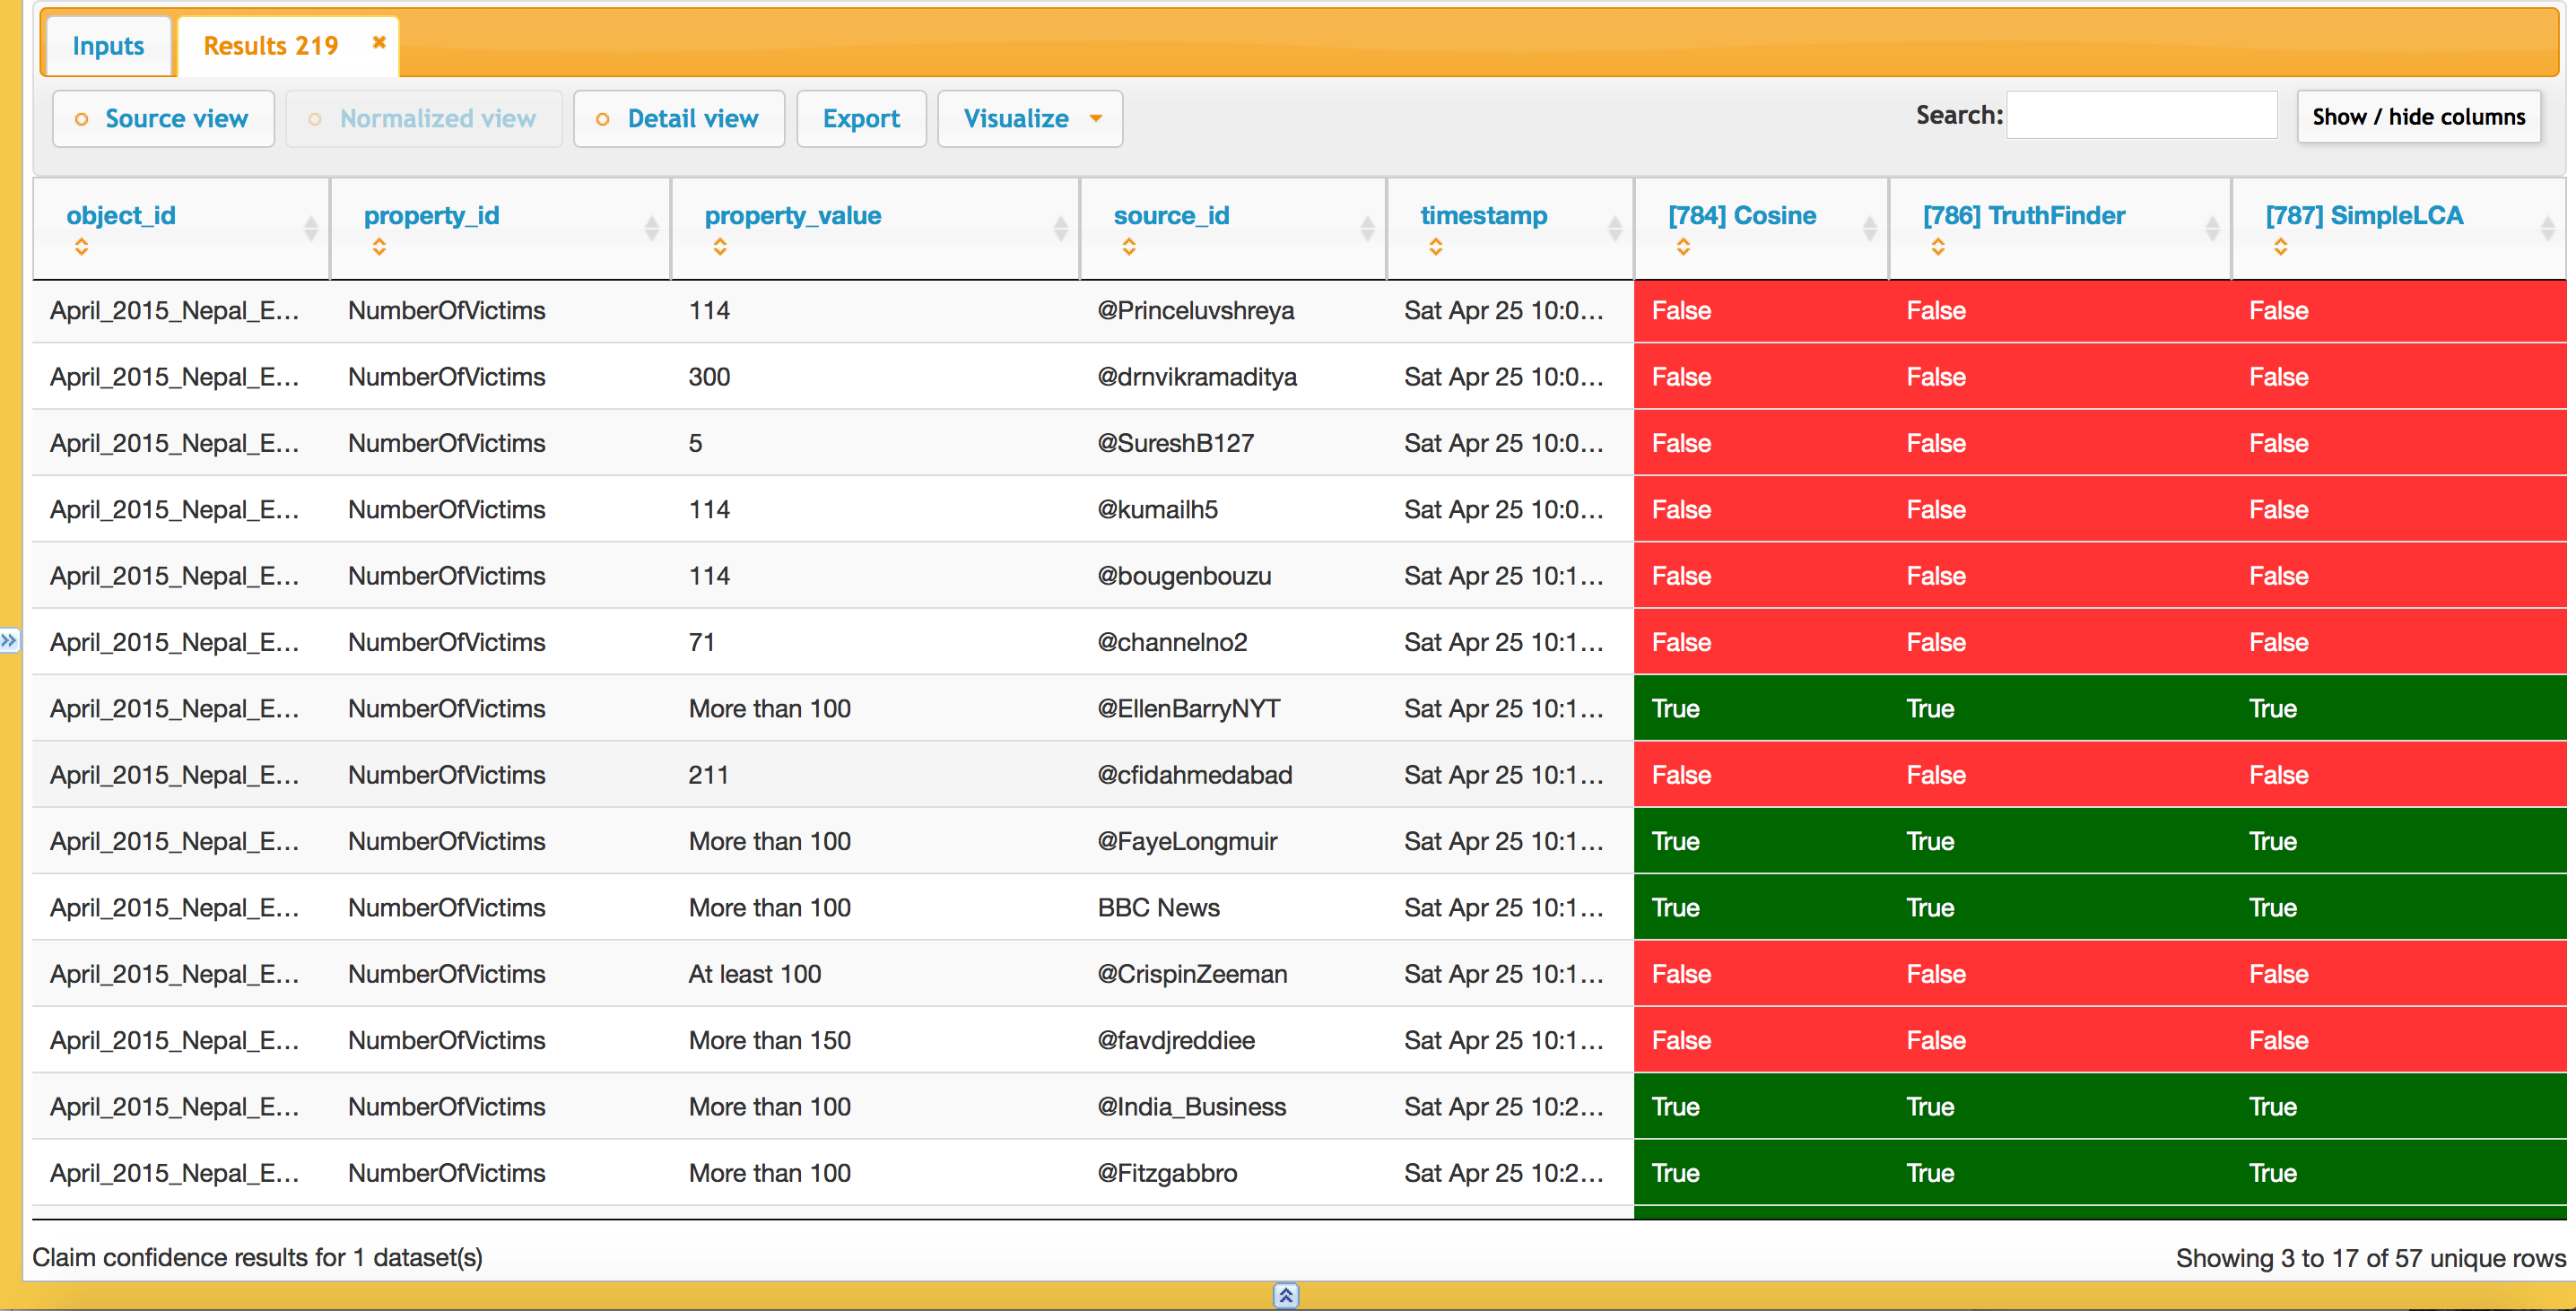
\includegraphics[width=.75\linewidth]{screenshot.png}
   \end{center}
\label{screenshot}\caption{$\VERA$: Behind the Scene}
\end{figure*}

\section{demonstration scenarios}
During the demo we will show how $\VERA$  estimates the veracity
of multi-source information from  Web sources and tweets.
The audience will see two main truth discovery scenarios that can
not be accomplished using conventional search engines or existing
truth discovery methods and we will show how they can be handled
using $\VERA$.


\textbf{Real-Time Fact-Checking for Crisis Situations.}
In crisis situations, time is critical when  an emergency response must be issued as soon as possible. Often the only information the public receives about the situation or the disaster is through the media (usually by authoritative sources) only once it is verified and but also immediately through social media as volunteered information that still needs to be checked. In this demonstration scenario,  $\VERA$ is combined to AIDR~\cite{AIDR} to estimate the veracity of  claims extracted from the content of tweets. Figure 3 presents  $\VERA$ behind the scene and shows the results of multiple truth discovery methods. These methods have been applied to the claims extracted  by TwitIE and structured by $\VERA$ from a collection of tweets related to Nepal earth quake  on April 25, 2015 in the time window 10:06AM--10:23AM as presented in the figure; the tweets were classified through AIDR in the category \textquote{injured or dead people}. As the time goes by, more information corroborate the true number of casualties. $\VERA$ source view  also provides the trustworthiness scoring  and ranking of the sources (twitter ids and Web sources) evolving in time.


\textbf{Rumors.} Nowadays, rumors about facts related to persons (e.g., celebrities) or hot events are ubiquitous on the Web.
Some rumors are purposely propagated for misinformation or propaganda, (e.g., Barack Obama is born in Kenya) and others are tied to a certain context which requires to have more information as soon as possible to confirm or deny them (e.g., the rumor of the bombing of \textquote{Les Halles shopping center} during Paris attacks in November 2015). Such kinds of rumors often spread out very quickly in  social media due to the lack of effective means to detect them. This scenario will show how $\VERA$ operates on rumors  by leveraging the sources' trustworthiness and time-dependent consensus in truth discovery computation.

